\documentclass{CST_CryptoIntro}
\usepackage{indentfirst}
% ===== 封面配置 =====
\reportCourse{密码分析学实验报告}
\reportLogo{figures/logo_sduWithText.jpg}
\reportName{邱泽辉、江李阳、王健一}
\reportID{202400460046、202400460042、202400460037}
\reportMajor{密码科学与技术}

% ===== 页眉配置 =====
\headerLeft{密码分析学}
\headerRight{第一次实验实验报告}

\begin{document}

% ===== 封面 =====
\maketitle
\thispagestyle{fancy}
\newpage

% ===== 目录 =====
\tableofcontents
\newpage

% ================================================================
% 正文内容
% ================================================================
\section{实验目的}

本实验围绕 Enigma 密码机的结构、加密过程和密钥空间展开。通过编程实现给定参数下的 Enigma 加密，理解接线板、转子和反射器在密码变换中的作用；在此基础上分析转子排列、转子起始位置和接线板设置所形成的密钥空间，并结合实际加密速度判断直接穷举攻击的可行性。

\subsection{组员分工}
\begin{itemize}
    \item 邱泽辉（202400460046）：任务一、任务二的实现以及任务二的撰写。
    \item 江李阳（202400460042）：任务一、任务三的实现以及报告主体的撰写。
    \item 王健一（202400460037）：任务二的实现以及报告的补充、修改与整合。
\end{itemize}
% 实验环境
\section{实验环境}

本实验在个人计算机上完成，使用 Python 编写 Enigma 密码机的模拟和性能测试程序。具体环境如下：

\begin{itemize}
    \item 硬件环境：13th Gen Intel(R) Core(TM) i5-13420H 处理器，12 个逻辑处理器，主频约为 2.1 GHz；内存 16 GB。
    \item 软件环境：Windows 操作系统、MacOS,Visual Studio Code 集成开发环境。
    \item 编程语言：Python 3.14。
\end{itemize}


%实验原理
\section{实验原理}

\subsection{字母与置换表示}

本实验将 26 个英文字母按照 $A=0,B=1,\ldots,Z=25$ 编码。接线板、转子和反射器都可以看作字母集合上的置换。若一个部件将输入字母对应到输出字母，则可以用一个长度为 26 的数组表示该置换。

\subsection{Enigma机的加密结构}
\begin{figure}[H]
    \centering
    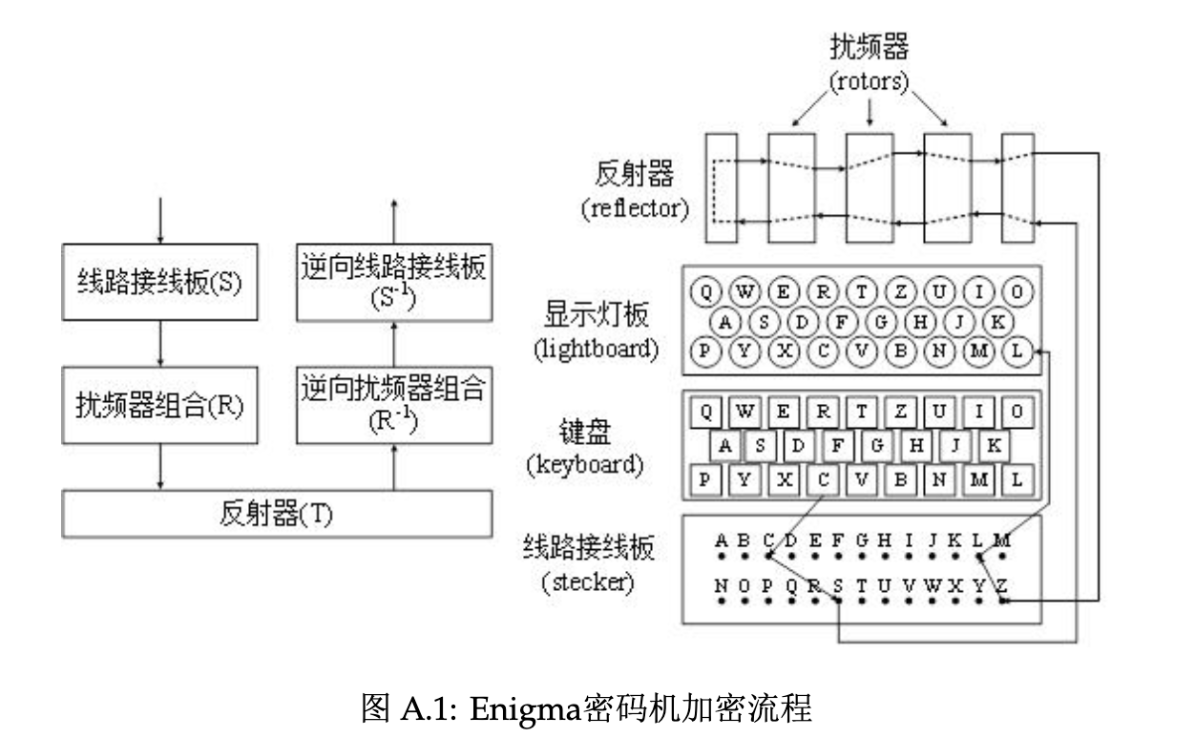
\includegraphics[width=0.8\textwidth]{figures/Enigma.png}
    \caption{Enigma机的结构}
    \label{fig:Enigma}
\end{figure}
Enigma 机主要由接线板、转子组和反射器组成。设接线板置换为 $S$，三个转子在当前状态下共同形成的正向变换为 $R_i$，反射器置换为 $T$。其中下标 $i$ 表示正在处理第 $i$ 个字符时的转子状态。

对于明文字符 $P_i$，其加密过程为：先经过接线板，再依次通过三个转子和反射器，随后沿相反方向通过三个转子的逆变换，最后再次经过接线板。因此有

\begin{equation*}
    C_i=S^{-1} \circ R_i^{-1} \circ T \circ R_i \circ S(P_i).
\end{equation*}

式中，$S^{-1}$ 表示接线板的逆置换，$R_i^{-1}$ 表示当前转子组的逆变换，$T$ 表示反射器。反射器满足$T(\alpha) = \beta,\alpha \neq \beta$,即反射器的输入与输出必然不相等。这导致了Enigma具有密文字母一定与明文字母不同的特点：
令
$$
C = E(P) = S^{-1} \circ R^{-1} \circ T \circ R \circ S(P)
$$
假设存在$P = E(P)$，代入上式可得:
$$
P = S^{-1} \circ R^{-1} \circ T \circ R \circ S(P) \Rightarrow \\
R \circ  S(P) = T \circ R \circ S(P)
$$
令$ R \circ S(P) = \gamma $，上式得到:
$$
\gamma = T(\gamma)
$$
这与反射器的定义相矛盾，因此假设不成立，不存在$P$使得$P = E(P)$，这一特殊事件是后续对Enigma机破解的一个利用点。

\subsection{接线板}

接线板密钥记为 $K_1$。每条接线连接两个不同字母，使两个字母互相交换；没有接线的字母映射到自身。若接线板恰好有 $l$ 条接线，先从 26 个字母中选出参与接线的 $2l$ 个字母，再将其两两配对，因此可能的接线板数量为

\begin{equation*}
    N_{K_1}(l)=\binom{26}{2l}\frac{(2l)!}{2^l l!}
    =\frac{26!}{(26-2l)!2^l l!}.
\end{equation*}

其中 $2^l$ 用于消除每条接线两端交换所造成的重复计数，$l!$ 用于消除不同接线之间排列顺序造成的重复计数。按照参考程序中“不超过 6 条接线”的限制，严格的接线板密钥数量为

\begin{equation*}
    N_{K_1,\leq 6}=\sum_{l=0}^{6}N_{K_1}(l)
    =105\,578\,918\,576\approx2^{36.62}.
\end{equation*}

若只取接线数量最大的情况 $l=6$ 进行数量级估计，则

\begin{equation*}
    N_{K_1}(6)=\frac{26!}{14!2^6 6!}
    =100\,391\,791\,500\approx2^{36.55}.
\end{equation*}

\subsection{转子组与转动规则}

转子内部的连线是预先固定的，但转子的安装顺序和起始位置会改变整体置换。在任务一中，三个转子的顺序固定为快速、中速、慢速转子 $(I,II,III)$，起始位置为 $(8,9,10)$。每处理一个明文字符后，快速转子向前转动一个位置；快速转子转满 26 次后，中速转子转动一个位置；中速转子转满 26 次后，慢速转子转动一个位置。

若三个转子的集合固定但顺序未知，则转子顺序有 $3!$ 种选择，每个转子的起始位置有 26 种选择，因此转子密钥数量为

\begin{equation*}
    N_{K_2}=3!\times26^3=105\,456\approx2^{16.69}.
\end{equation*}

实际使用的Enigma机中为了增大$K_2$的密钥空间，通常会从$t$个备选转子中选择$3$个，并按照一定初始化顺序组成实际在用的扰频器，此时该密钥的数量为:
\begin{equation*}
    N_{K_2}  =  P_t^3 \times 26^3
\end{equation*}

在任务三中，从 4 个转子中选择 3 个并安排到快速、中速、慢速三个位置

因此任务三的转子密钥数量为

\begin{equation*}
    N_{K_2}'=P_4^3\times26^3=421\,824\approx2^{18.69}.
\end{equation*}


%实验内容

\section{任务一}

本任务要求寻找除题目给定差分之外的高概率四轮差分。题目给出的差分为
\[
    (0x0,0x0,0x0,0x1)
    \xrightarrow{\text{4轮}}
    (0x0,0x0,0x0,0x1),
\]
也可以写成
\[
    0x0001\xrightarrow{\text{4轮}}0x0001.
\]

\subsection{直接穷举思路}

对于固定的输入差分 $\alpha$，可以遍历所有 $2^{16}$ 个 16 比特明文 $x$，构造有序明文对 $(x,x\oplus\alpha)$，然后分别进行四轮 CipherFour 加密。若最终密文差分为 $\beta$，则将对应计数加一。因此，固定输入、输出差分的概率为
\[
    P(\alpha\rightarrow\beta)
    =
    \frac{\#\{x:E(x)\oplus E(x\oplus\alpha)=\beta\}}{2^{16}}.
\]

对于每一个非零输入差分，共有 $2^{16}$ 个有序明文对；如果不区分明文对的顺序，则有 $2^{15}$ 个无序明文对。若对全部 $2^{16}-1$ 个非零输入差分都进行穷举，需要处理约 $2^{32}$ 组明文对，计算开销较大。因此，程序使用 S 盒差分分布表（DDT）对差分进行动态规划。

\subsection{S盒差分分布表}

CipherFour 使用一个 4 进 4 出的 S 盒。对于输入差分 $\alpha$ 和输出差分 $\beta$，DDT 定义为
\[
    \mathrm{DDT}[\alpha][\beta]
    =
    \#\left\{x\in\{0,1,\ldots,15\}:
    S(x)\oplus S(x\oplus\alpha)=\beta\right\}.
\]

因此，单个 S 盒的差分传播概率为
\[
    T[\alpha][\beta]
    =
    \frac{\mathrm{DDT}[\alpha][\beta]}{16}
    =
    \frac{\mathrm{DDT}[\alpha][\beta]}{2^4}.
\]

代码中的 DDT 计算如下：
\begin{lstlisting}
for diff_in in range(16):
    for value in range(16):
        diff_out = S[value] ^ S[value ^ diff_in]
        diff_table[diff_in][diff_out] += 1
\end{lstlisting}

其中，\texttt{diff\_table[diff\_in][diff\_out]} 保存输入差分为 \texttt{diff\_in}、输出差分为 \texttt{diff\_out} 的出现次数。

\subsection{一轮差分传播}

一个 16 比特差分可以拆成四个半字节：
\[
    \Delta=(a_0,a_1,a_2,a_3).
\]

若四个 S 盒的输出差分为
\[
    \Gamma=(b_0,b_1,b_2,b_3),
\]
则在固定当前差分的条件下，四个 S 盒同时发生该传播的概率为
\[
    Q(\Delta,\Gamma)
    =
    \prod_{i=0}^{3}T[a_i][b_i].
\]

例如，输入差分 $0x0001=(0,0,0,1)$ 时，前三个 S 盒的输入差分为 0，并且
\[
    T[0][0]=1.
\]
只有最后一个 S 盒产生分支。对于本实验使用的 S 盒，输入差分 1 可以传播为输出差分 1、2、5，其概率分别为 $1/2$、$1/4$、$1/4$。因此，经过 S 盒层后可能得到
\[
    0x0001\ (1/2),\qquad
    0x0002\ (1/4),\qquad
    0x0005\ (1/4).
\]

代码中的 \texttt{score} 保存四个半字节的联合概率分布，其形状为
\[
    (\text{batch},16,16,16,16).
\]
处理某一个半字节时，程序计算
\[
    F_{\mathrm{new}}(\beta)
    =
    \sum_{\alpha=0}^{15}
    F_{\mathrm{old}}(\alpha)T[\alpha][\beta].
\]

这对应代码中的矩阵乘法：
\begin{lstlisting}
score_matrix = moved_score.reshape(-1, 16)
updated_score = score_matrix @ probability_table
\end{lstlisting}

程序依次处理四个 S 盒：
\begin{lstlisting}
for position in range(4):
    score = update_one_sbox_distribution(
        score, probability_table, position
    )
\end{lstlisting}

对于一个确定的当前 16 比特差分，这一过程等价于四个 S 盒概率的乘积；当当前状态本身是多个差分状态的概率混合时，程序还会对所有前驱状态的概率进行求和，因此需要保存四个半字节的联合分布，而不能只分别保存四个边缘概率。

四个 S 盒处理完成后，将得到的 16 比特差分经过 P 置换。代码预先计算所有 16 比特状态的置换结果：
\begin{lstlisting}
permutation = np.array(
    [P_box(value) for value in range(STATE_SIZE)],
    dtype=np.int32,
)
\end{lstlisting}

由于 P 是比特置换，满足
\[
    P(X)\oplus P(Y)=P(X\oplus Y),
\]
因此可以直接对差分状态进行 P 置换。经过 P 置换后的差分分布作为下一轮的输入。

\subsection{四轮动态规划}

设初始输入差分为 $\alpha$，经过 $r$ 轮后的差分分布为 $D_r^{(\alpha)}$。初始时只有输入差分本身的概率为 1：
\[
    D_0^{(\alpha)}(\Delta)=
    \begin{cases}
        1,&\Delta=\alpha,\\
        0,&\Delta\ne\alpha.
    \end{cases}
\]

代码通过以下语句完成初始化：
\begin{lstlisting}
score[rows, nibble0, nibble1, nibble2, nibble3] = 1.0
\end{lstlisting}

记一轮四个 S 盒和 P 置换的差分转移概率为 $R(\Delta,\Delta')$，则每轮动态规划满足
\[
    D_{r+1}^{(\alpha)}(\Delta')
    =
    \sum_{\Delta}
    D_r^{(\alpha)}(\Delta)R(\Delta,\Delta').
\]

因此，四轮后的输出差分概率为
\[
    D_4^{(\alpha)}(\beta)
    =
    \sum_{\Delta_1,\Delta_2,\Delta_3}
    R(\alpha,\Delta_1)
    R(\Delta_1,\Delta_2)
    R(\Delta_2,\Delta_3)
    R(\Delta_3,\beta).
\]

这个求和包含了从输入差分 $\alpha$ 到输出差分 $\beta$ 的所有差分路线。代码的外层循环对应四轮传播：
\begin{lstlisting}
for _ in range(NUMBER_OF_ROUNDS):
    for position in range(4):
        score = update_one_sbox_distribution(
            score, probability_table, position
        )

    after_sbox = score.reshape(batch_size, STATE_SIZE)
    after_pbox[:, permutation] = after_sbox
    score = after_pbox.reshape(
        batch_size, 16, 16, 16, 16
    )
\end{lstlisting}

这里每一轮的输入和输出都是 16 比特差分状态的概率分布，不是具体的明文或密文。四轮循环结束后，\texttt{score} 中保存每个输入差分经过四轮后得到所有输出差分的概率。

\subsection{高概率差分的搜索}

程序从 \texttt{0x0001} 到 \texttt{0xFFFF} 遍历全部 $2^{16}-1$ 个非零输入差分，并将输入差分按 32 个一批进行处理，以降低内存开销。分批处理不会减少搜索范围。

对于每个输入差分 $\alpha$，四轮动态规划得到所有输出差分 $\beta$ 的概率分布。程序使用
\begin{lstlisting}
output_differences = np.argmax(
    output_distribution, axis=1
)
\end{lstlisting}
找到该输入差分对应的最大概率输出差分。随后，再在所有输入差分对应的候选结果中选择全局最大值。

题目要求排除 $0x0001\rightarrow0x0001$，因此代码只对输入差分 \texttt{0x0001} 的输出分布执行：
\begin{lstlisting}
candidate_distribution[
    EXCLUDED_OUTPUT_DIFFERENCE
] = 0.0
\end{lstlisting}
然后重新选择该输入差分对应的最佳输出差分。

\begin{figure}[H]
    \centering
    
\includegraphics[width = 1\textwidth]{figures/task1_diffeientrial.png}
    \caption{寻找高概率差分}
\end{figure}

程序最终找到的四轮高概率差分为
\[
    (0x0,0x0,0x0,0x1)
    \longrightarrow
    (0x0,0x0,0x1,0x0),
\]
即
\[
    0x0001\longrightarrow0x0010.
\]

其基于 DDT 动态规划得到的四轮差分概率为
\[
    P(0x0001\rightarrow0x0010)
    =0.0479736328125
    \approx 2^{-4.381614}.
\]

这里计算的是连接相同输入、输出差分的所有差分路线的概率总和，而不是某一条单独差分路线的概率。后续任务二再通过枚举具体明文对，统计该输入、输出差分在固定 CipherFour 置换网络中的实际路线和频率。
\section{任务二}
给定如下明密文数据流，任务1中的三个转子和反射器的定义不变，但转子顺序不固定，请尝试恢复密钥K1和K2。（假设加密过程中，中速和慢速转子不转动）

明文WETTERVORHERSAGEHEUTE

密文EWGZDSATLWNEDBBCJUNGW

\subsection{思路分析}
\subsubsection{分割密钥空间}
实验给的明文和密文长度一样，且没有出现明文字母和密文字母相同的情况，因此可以认为这就是对应的明密文，即Crib，

由于加密的时候密钥K1和K2是合并起来的，穷举数量太大，因此需要分割密钥空间，我们可以类比2-DES的攻击，通过一些相同的中间量来脱去外层加密,把\(K_1\)和\(K_2\)分开

前面探讨过，\(|K_1| >> |K_2|\),所以我们寄希望于消除掉\(K_1\),先回复\(K_2\)

\subsubsection{寻找中间状态}
我们注意到这样的一种特殊的Crib，即内部能形成环路的Crib，因为接线板就是一个由连接线决定的单表代换，这个过程和K2没有关系，
enigma机的明文输入会经过一次接线板，而输出密文前也会经过一次接线板，这之间有一个中间状态。
我们就可以利用这个中间状态单独回复\(K_2\)，然后再去恢复\(K_1\)，实现对于密钥空间的分割，降低密钥恢复的复杂度。

以课程上的一个crib为例，
\begin{figure}[H]
    \centering
    
\includegraphics[width=0.8\textwidth]{figures/crib.png}
    \caption{Crib}
    \label{fig:Crib}
\end{figure}
明文里的W,经过接线板，\(K_1\)我们可以理解成一个可逆的单表带换，即\(K_1(W)=L_0\)，

然后密文的E，\(K_1(E)=L_1\)，此时我们发现明文的下一个也是E，它得到的中间状态也应该是\(L_1\),那这样我们就能消解掉接线板的影响

(值得注意的是，这里的Crib是一种交替的环路，就是从明文-密文-明文-密文...这样明密文交替进行的，这实际上会影响后续的数据结构，参考程序中并不是这样的，不过这又是后话了)
\subsubsection{建立关于\(K_2\)的方程}
我们利用这个中间状态来建立K2的方程：
它有一个\textbf{不随机现象}就是，\(L_0\)进\(L_0\)出，
而\(L_1\)本身就是\(L_0\)经过扰频器和反射器得到的，也就是说，知道\(L_0\)和\(K_2\),就能计算\(L_1,L_2\)
\[
L_{i-1} \xrightarrow{K_2} L_i
\]
我们简单把这个步骤记作\({Enc}_{K_2}\)
因此这中间的路径也被消解了，我们只需要关注首尾的\(L_0\),正确的K2应该能让\(L_0\)进\(L_0\)出

我们只需要遍历\(|K_2|\times|L_0|\)次，其中\(|L_0|=26\),这远远小于\(|K_1|\times|K_2|\)的穷举
当然这个也会有错误，但是我们多找几个环路，然后取交集，就能得到比较少的候选了。

其中对中间状态而言，正确的$K_2$必然满足$L_0$进且$L_0$出；对于错误的$K_2$，我们将环路看作随机置换，输入为$i,i \in \{A,B,\dots,Z\}$，输出为$\pi(i)$。满足环路即
$$
i = \pi(i)
$$
这里随机置换共$26!$种，结合错排数公式:
$$
D_n = n! \sum_{k=0}^n \frac{(-1)^k}{k!}
$$
得到错排率为
$$
Pr = \frac{D_{26}}{26!} = \sum_{k=0}^{26} \frac{(-1)^k}{k!} = 1 - 1 + \frac{1}{2!} -\frac{1}{3!}+...+\frac{1}{26!}
$$
利用$e^{-x}$的泰勒展开式：
$$
e^{-x} = \sum_{k=0}^{\infty}\frac{(-1)^k x^k}{k!}
$$
因此有$ Pr \approx e^{-1}  $。回到错误密钥但依然能形成环路的情况，即随机置换全部错排的对立面，对应概率为:
$$
Pr' = 1- Pr = 1- e^{-1} \approx 63.2\%
$$
可见错误率还是挺高的，需要结合后续其他条件筛掉错误密钥$K_2$。


当然这个也会有错误，但是我们多找几个环路，然后取交集，就能得到比较少的候选了
\subsubsection{根据环路恢复\(K_1\)以及\(K_2\)}
我们前面找到的可能的\(K_2\)的候选集，记为\(\{(L_0^{1i},K_2^1),(L_0^{2i},K_2^2),..., (L_0^{ni},K_2^n)\}\)
因为一个\(K_2\)可能对应多个\(L_0\),所以\(L_0^{1i},K_2^1\)可能有多个\(i\),即多个\(L_0\)对应同一个\(K_2\)
我们可以利用这些候选的\(K_2\)来恢复\(K_1\)，同时进一步筛选\(K_2\)
因为我们已知环路，比如W-E-E-T-T-W
那么就有\(K_1(W)=L_0\)，\(K_1(E)=L_1\)，\(K_1(T)=L_2\)，以此类推。
如何筛选呢？就是寻找矛盾，再回到完整的Crib，寻找\(K_1\)中已经有的字母，比如又找到一个W，它又会对应一个新的密文字母比如J

分两种情况
\begin{itemize}
    \item 如果J已经在\(K_1\)中出现过了，那么我们检查\({Enc}_{K_2}(K_1(W)) = K_1(J)\),如果不等，就排除这个\(K_1\),如果所有\(K_1\)都被排除，就排除这个\(K_2\)
    \item 如果J没有出现过，那么就可以继续扩展\(K_1(J) = {Enc}_{K_2}(K_1(W))\)
\end{itemize}
经过这轮筛选之后，我们就能恢复出\(K_1\)和\(K_2\)了
运行decrypt.py即可得到结果
\begin{figure}[H]
    \centering
    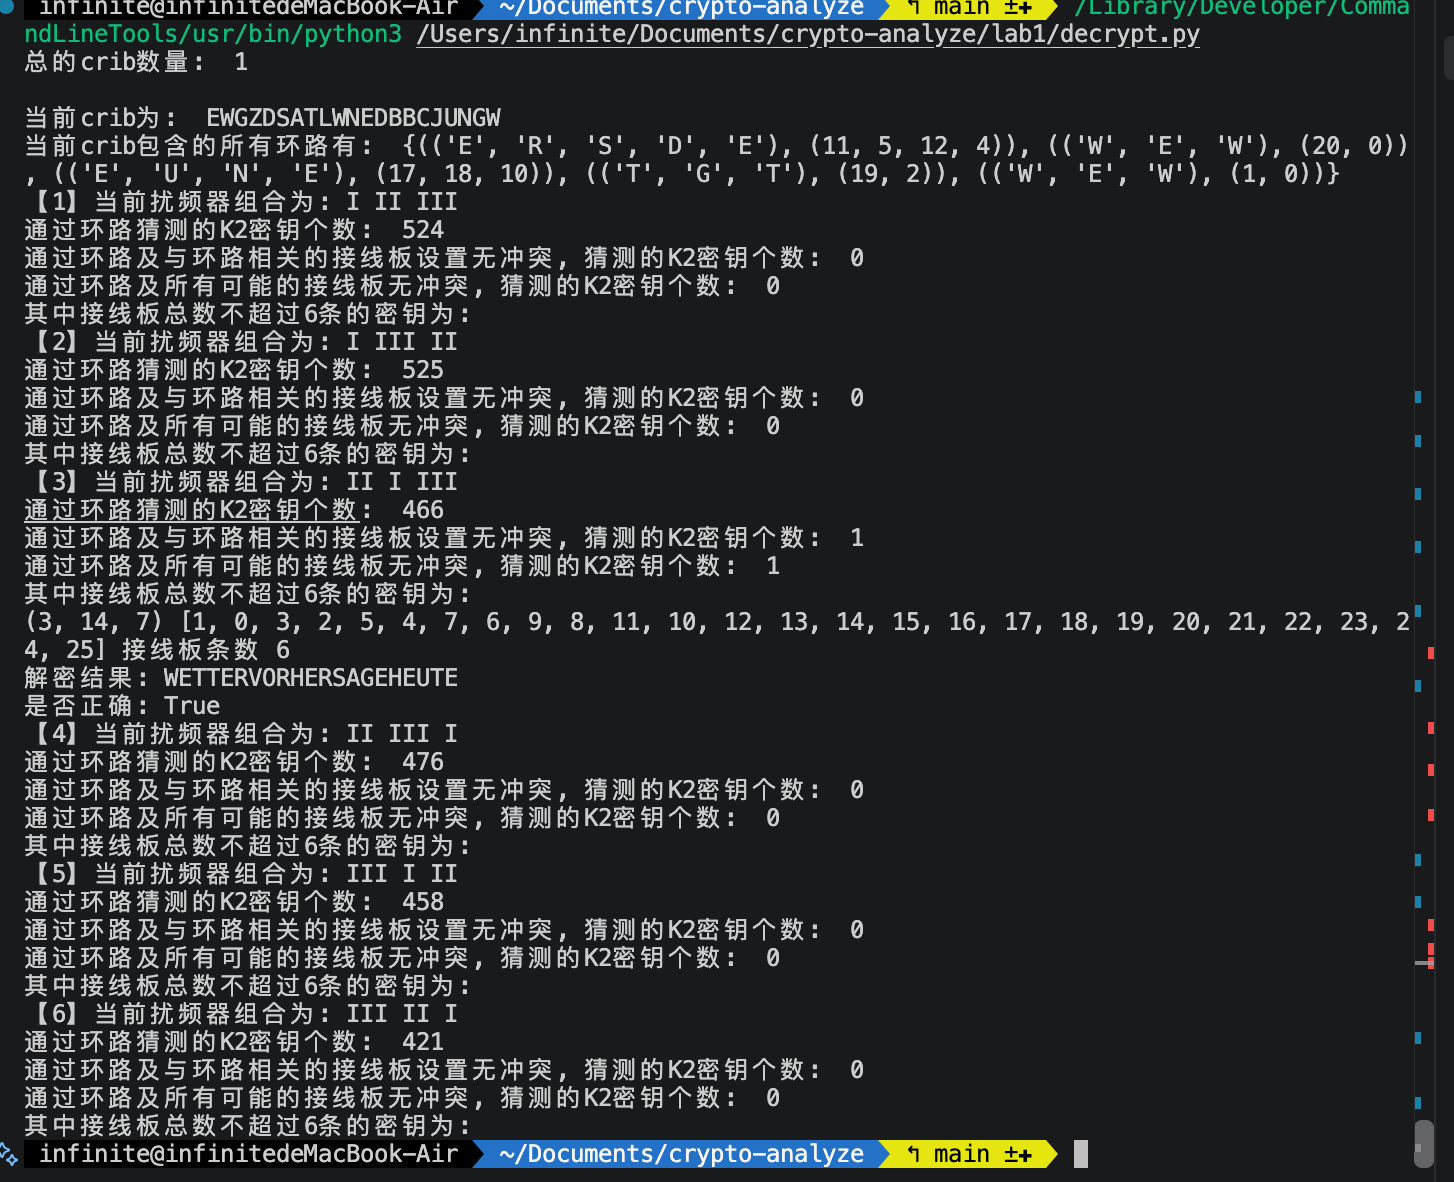
\includegraphics[width=0.8\textwidth]{figures/result3.png}
    \caption{result}
    \label{fig:res}
\end{figure}
最后\(K_1\)，\(K_2\)恢复的结果是：
\[
K_1=[1, 0, 3, 2, 5, 4, 7, 6, 9, 8, 11, 10, 12, 13, 14, 15, 16, 17, 18, 19, 20, 21, 22, 23, 24, 25]
\]

\[
K_2 = ((3, 14, 7),(II,I,III))
\]


\section{任务三}


\input{content/4summary.tex}
\appendix
\section{实验代码}
% \input{content/6note.tex}


% \section{参考资料}
% \begin{enumerate}
%     \item 《密码分析学实验一》实验指导书。
%     \item 课程课件《密码分析学概述》和《恩尼格玛密码机的破解》。
%     \item 实验目录中的 Enigma 参考程序，并在报告任务一中对相应参考内容作出说明。
% \end{enumerate}

\end{document}
